% $Id: parameter.tex,v 1.14 2009/11/21 09:23:25 baum Exp $
% Tag $Name: tinyheb-1-6-3 $


% Copyright (C) 2004 - 2013 Thomas Baum <thomas.baum@arcor.de>
% Thomas Baum, 42719 Solingen, Germany

% This program is free software; you can redistribute it and/or modify
% it under the terms of the GNU General Public License as published by
% the Free Software Foundation; either version 2 of the License, or
% (at your option) any later version.

% This program is distributed in the hope that it will be useful,
% but WITHOUT ANY WARRANTY; without even the implied warranty of
% MERCHANTABILITY or FITNESS FOR A PARTICULAR PURPOSE.  See the
% GNU General Public License for more details.

% You should have received a copy of the GNU General Public License
% along with this program; if not, write to the Free Software
% Foundation, Inc., 59 Temple Place - Suite 330, Boston, MA 02111-1307, USA.


\chapter{Parameter\label{parameter:kap}}
\index{Parameter}
In diesem Kapitel werden die einzelenen Parameter beschrieben die
es in \tinyHeb\/ gibt. Wie neue Parameter angelegt, resp. geändert werden
können und insbesondere welche Ausprägungen sie besitzen und welche
steuernde Wirkung sie im Rest von \tinyHeb\/ haben. Die hier beschriebenen
Parameter haben eine zentrale Bedeutung für die Anwendung. Das heißt
insbesondere, dass durch Löschen von bestimmten Parametern die Anwendung
nicht mehr funktionsfähig sein kann. Also: Nur dann Parameter ändern,
wenn man weiss, welche Auswirkung die Änderung hat.
\marginline{\Huge\bfseries!}%

\section{Parametererfassung}
Aus dem Hauptmenue gelangt man, wie schon im Kapitel 
\vref{einleitung:parameter:kap} beschrieben über den Link 
\verb|weitere| \verb|Wartungspunkte| in das \tinyHeb\/ 
Wartungsmenue (Abbildung \vref{parameter:wartungsmenue:fig}) und von dort über den
Link \verb|alle| \verb|Parameter| in die Maske zur Parameterpflege 
(Abbildung \vref{parameterpflege:fig}).
%
\begin{figure}[h]
\centering
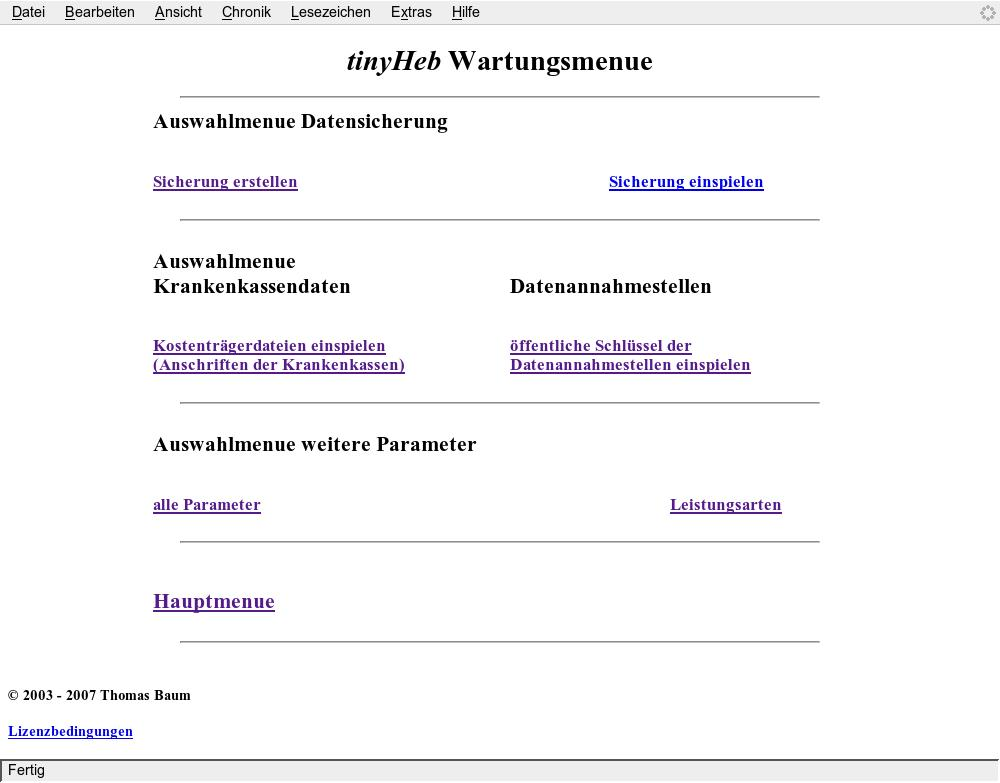
\includegraphics[width=80mm]{wartungsmenue}
\caption{\tinyHeb\/ Wartungsmenue \label{parameter:wartungsmenue:fig}}
\end{figure}
%
\begin{figure}[ht]
\centering
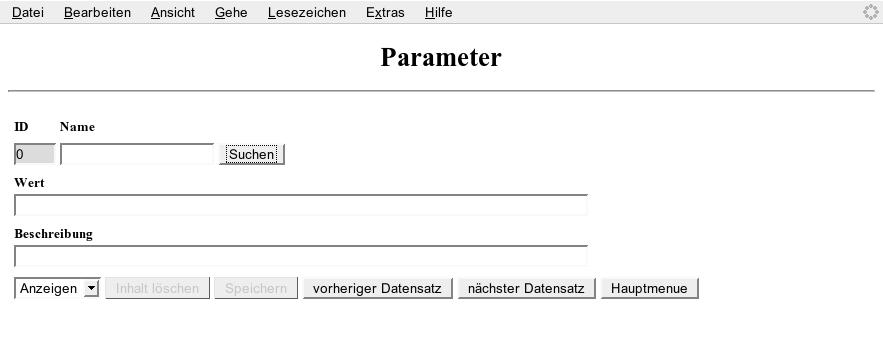
\includegraphics[width=80mm]{parameterpflege}
\caption{Parameterpflege\label{parameterpflege:fig}}
\end{figure}
%

Die Maske zur Pflege der Parameter ist relativ simple gestaltet. 
Folgende Felder sind in der Maske vorhanden:

\begin{description}
\item[ID] Dieses Feld enthält die interne ID zum angezeigten Parameter, es wird
automatisch gefüllt und kann nicht geändert oder erfasst werden.
\item[Name] Name des Parameters, über diesen Namen wird in der 
Anwendung auf den Wert des Parameters zugegriffen. Es ist auf korrekte 
Schreibweise (insb. Groß-/ Kleinschreibung) zu achten, da sonst nicht
auf den Wert zugegriffen werden kann. Es kann zwischen zwei Arten von
Namen unterschieden werden, eindeutige Namen, z.B. RECHNR, oder Namen, die 
häufiger vorkommen können, z.B. BEGRUENDUNG. Es exisiert keinerlei
Plausiprüfung für den Inahlt des Feldes.
\item[Wert] Dieses Feld enthält den Wert zu dem im Feld \feld{Namen}
bezeichneten Parameter. Es exisiert keinerlei Plausiprüfung für den 
Inahlt des Feldes.
\item[Beschreibung] 
Dieses Feld kann eine Beschreibung zu dem Parameter
enthalten, wie z.B. ``Zähler für Rechnungsnummer'' für das Feld RECHNR.
Es exisiert keinerlei Plausiprüfung für den Inahlt des Feldes.
\end{description}

\subsection{Beschreibung der Knöpfe im Parametermenue}
\begin{description}
\item[Suchen] Mit dem Knopf \knopf{Suchen} kann eine weitere Maske geöffnet
werden, über die Parameter gesucht werden können. Die Beschreibung zu der
Suchmaske befindet sich in Abschnitt \vref{parameterauswahl:abs}.
In diese Maske werden die Werte aus den Feldern \feld{Name, Wert} sowie
\feld{Beschreibung} übernommen und die Suche unmittelbar gestartet.
\item[Inhalt löschen] Der Knopf \knopf{Inhalt löschen} ist nur dann
Aktiv, wenn in dem
Pop Down Menue vor dem Knopf der Wert Neu ausgewählt wurde. Wird der Knopf
gedrückt, werden alle Felder der Maske auf ihren initalen Wert gesetzt und das
Pop Down Menue springt auf den Wert Anzeigen,
\item[Speichern/ Löschen] Der Knopf \knopf{Speichern} ist nur dann aktiv,
wenn im Auswahlmenue entweder der Wert Neu oder Ändern gewählt wird. 
\par
Falls Neu 
ausgewählt wurde, wird ein neuer Parametersatz in der Datenbank gespeichert
und das Pop Down Menue springt auf den Wert Anzeigen. Es finden wie
schon bei der Erfassung der Felder beschrieben keine Plausibilitäten
Prüfungen statt.\par
Falls Ändern gewählt wurde, wird der Datensatz, der sich in der Datenbank
befindet mit den angezeigten Werten überschrieben und das Pop Down Menue
springt auf den Wert Anzeigen. 
Es finden, wie
schon bei der Erfassung der Felder beschrieben, keine Plausibilitäten
Prüfungen statt.\par
Falls im Pop Down Menue Löschen ausgewählt wurde, erhält der Knopf die
Beschriftung Löschen. Durch Drücken des Knopfes wird der Datensatz aus der
Datenbank gelöscht. Es findet keine Plausiprüfung statt.
Wurde der Datensatz erfolgreich gelöscht, werden
alle Felder der Maske auf ihren Initial-Wert gesetzt und das Auswahlmenue
steht auf den Wert Anzeigen.
\item[vorheriger Datensatz] Dieser Knopf ist nur dann aktiv, wenn der Wert
des Pop Down Menues auf Anzeigen steht. Durch Drücken des Knopfes wird auf
den vorherigen Datensatz in der Datenbank gesprungen. Der vorherige Datensatz
ist derjenige mit der nächst kleineren ID, als der aktuell angezeigte. Ist
man am ersten Datensatz angekommen, bleibt dieser in der Maske erhalten.
\item[nächster Datensatz] Dieser Knopf ist nur dann aktiv, wenn der Wert
des Pop Down Menues auf Anzeigen steht. Durch Drücken des Knopfes wird auf
den nächsten Datensatz in der Datenbank gesprungen. Der nächste Datensatz
ist derjenige mit der nächst höheren ID, als der aktuell angezeigte. Ist
man am letzten Datensatz angekommen, bleibt dieser in der Maske erhalten.
\item[Hauptmenue] Über diesen Knopf gelangt man in die Maske Hauptmenue.
Dabei ist zu beachten, dass nicht überprüft wird, ob Änderungen oder Neu
erfasste Daten gespeichert wurden. Es wird sofort in die Maske Hauptmenue
gesprungen.
\end{description}

Sind alle Felder erfasst, können die Daten gespeichert werden. Dazu ist
es notwendig im Pop Down Menue unten links den Wert 'Neu' auszuwählen.
Sobald dies geschehen ist, wird der Knopf \knopf{Speichern} aktiv 
geschaltet. Drückt man jetzt den Knopf \knopf{Speichern} werden die Daten
zu dem Parameter permanent abgelegt. Nach dem Speichern wird die Auswahl im 
Pop Down Menue unten links auf den Wert 'Anzeigen' gesetzt.




\section{Parameterauswahl\label{parameterauswahl:abs}}
In diesem Absatz ist beschrieben, wie Parameter im Datenbestand gesucht und
ausgewählt werden können. Der  Aufruf der Maske erfolgt aus der 
Parametererfassung (siehe Seite \pageref{parameterpflege:fig}) 
über den Knopf \knopf{Suchen}. 
Klickt man auf den Knopf \knopf{Suchen} wird ein neues Fenster mit der
Überschrift ``Parameter suchen'' geöffnet\footnote{sollte das Fenster 
noch geöffnet sein, wird es in den Vordergrund des Bildschirms geholt.} 
(siehe Abbildung \vref{parameterauswahl:fig}). Über die Felder \feld{Name,
Beschreibung, Wert} ist es möglich die
Suchkrieterien vorzugeben, d.h. es werden bei der Suche nur die Parameter
ausgegeben, bei denen alle vorgegebenen Werte vorhanden sind. Dabei ist
folgendes für die Felder zu beachten:

\begin{figure}[ht]
\centering
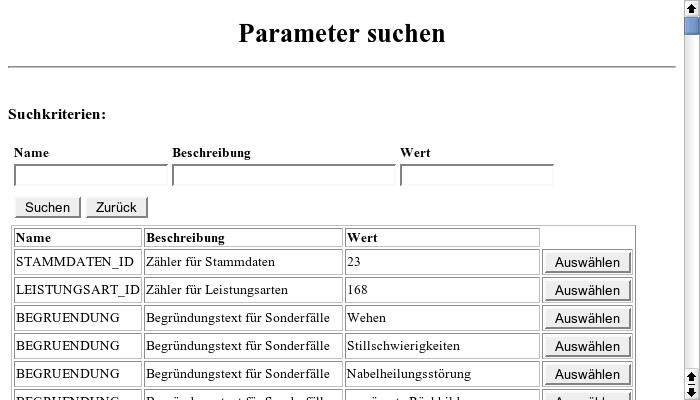
\includegraphics[width=9cm]{parameterauswahl}
\caption{Parameterauswahlmaske\label{parameterauswahl:fig}}
\end{figure}

\begin{description}
\item[Name] Es wird nur nach den Parametern gesucht, bei denen der Name
einen Teil des Feldes enthält.
Wird z.B. im Feld \feld{Name} ``HEB'' erfasst,
würde HEB\_VORNAME, HEB\_NACH\-NAME, HEB\_PLZ, usw. ermittelt werden.
\item[Beschreibung] Es wird nur nach den Parametern gesucht, bei denen die
Beschreibung mit dem Feldinhalt beginnt. Wird z.B. im Feld 
\feld{Beschreibung} ``Zähler'' erfasst,
würden alle Parameter, die mit ``Zähler'' beginnen ermittelt werden, d.h.
``Zähler für Stammdaten'', ``Zähler für Leistungsarten'', usw.
\item[Wert] Es wird nur nach den Parametern gesucht, die diesen Wert
enthalten.
\end{description}

Ist der Aufruf der Maske aus der Maske Parameter
erfolgt, werden die Werte Name, Wert und Beschreibung
in die Suchkriterien übernommen und die Suche wird unmittelbar gestartet.
Die Felder können jederzeit mit neuen Suchkriterien gefüllt und die Suche
über den Knopf \knopf{Suchen} gestartet werden.

Das Ergebnis der Suche wird unmittelbar unter den Suchkriterien ausgegeben.
Es werden die Daten zu Name, Beschreibung und Wert ausgegeben.

Über den Knopf \knopf{Auswählen} werden die Daten des Parameters in die Maske
übernommen, aus der die Suchfunktion aufgerufen wurde. Die Maske
``Parameter suchen''
wird danach geschlossen.

Falls keine Parameter den gewünschten Suchkriterien entsprechen, kann entweder
durch Klicken des Knopfes \knopf{Zurück} die Maske ``Parameter suchen''
geschlossen werden, oder es können andere Suchkriterien erfasst werden.

\section{Beschreibung der einzelnen Parameter}

\subsection{Angaben zur Hebamme\label{parm:heb:abs}}
\index{Angaben zur Hebamme}
\index{Hebamme}
\index{Hebamme!IK-Nummer}
\index{Hebamme!Steuernummer}
\index{Steuernummer|see{Hebamme!Steuernummer}}
\index{Beleghebamme}
Die in Tabelle \vref{angaben_hebamme} beschriebenen Parameter lassen 
sich neben der Pflege in der Maske Parameter auch über die Maske
Angaben zur Hebamme ändern (siehe Abbildung \vref{angaben_zur_hebamme:fig}),
die über einen Link mit der identischen
Bezeichnung aus dem Hauptmenue erreichbar ist. Diese Maske enthält
alle relevanten Daten auf einen Blick.

\begin{figure}[H]
\centering
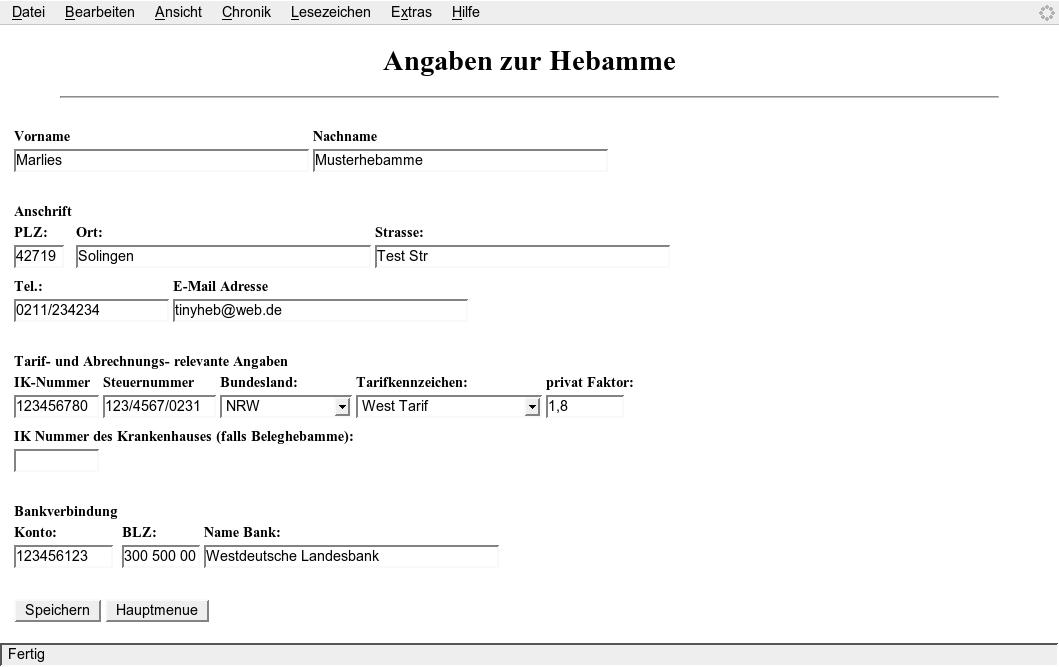
\includegraphics[width=80mm]{angaben_zur_hebamme}
\caption{Maske Angaben zur Hebamme\label{angaben_zur_hebamme:fig}}
\end{figure}


\bottomcaption{Angaben zur Hebamme\label{angaben_hebamme}}
\tablehead
{\hline \bfseries Name&\bfseries Beschreibung\\ \hline}

\tabletail
{\hline \multicolumn{2}{r}{\emph{Fortsetzung auf der nächsten Seite}}\\}

\tablelasttail{\hline}

\begin{mpsupertabular}{|p{3.9cm}p{9.0cm}|}
%\firsthline
%\textbf{Name}&\textbf{Beschreibung}
%\tabularnewline\hline
HEB\_VORNAME&
Vorname der Hebamme. Wird in die elektronische Rechnung übernommen und
auf der Papierrechnung mit angedruckt.
\tabularnewline\hline
HEB\_NACHNAME&
Nachname der Hebamme. Wird in die elektronische Rechnung übernommen und
auf der Papierrechnung mit angedruckt.
\tabularnewline\hline
HEB\_TEL&
Telefonnumer der Hebamme. Wird in die elektronische Rechnung übernommen und
auf der Papierrechnung mit angedruckt.
\tabularnewline\hline
HEB\_STRASSE&
Straße der Anschrift der Hebamme. Wird auf der Papierrechnung mit angedruckt.
\tabularnewline\hline
HEB\_PLZ&
Postleitzahl der Anschrift der Hebamme. Wird auf der Papierrechnung mit angedruckt.
\tabularnewline\hline
HEB\_ORT&
Ort der Anschrift der Hebamme. Wird auf der Papierrechnung mit angedruckt.
\tabularnewline\hline
HEB\_IK&
\index{Hebamme!IK-Nummer}
IK Nummer der Hebamme. Wird in die elektronische Rechnung übernommen und
auf der Papierrechnung mit angedruckt. Die IK Nummer wird in die Betreff
Zeile der E-Mail und in die ``Absender'' Zeile übernommen.
\tabularnewline\hline
HEB\_Konto&
Kontonummer der Hebamme. Wird auf der Papierrechnung mit angedruckt.
\tabularnewline\hline
HEB\_BLZ&
Bankleitzahl der Kontoverbindung der Hebamme. Wird auf der Papierrechnung
mit angedruckt.
\tabularnewline\hline
HEB\_NAMEBANK&
Bezeichnung der Bank, der Kontoverbindung der Hebamme. Wird auf der
Papierrechnung mit angedruckt.
\tabularnewline\hline
HEB\_TARIFKZ&
\index{Tarifkennzeichen}
Tarifkennzeichen der Hebamme gemäß \cite{schluessel}[Abschnitt 8.1.5.2].
Für Hebammen in Westdeutschland muss 24 eigetragen werden, für Hebammen
in Ostdeutschland 25, oder man benutzt 00 für bundeseinheitlichen Tarif.
Wird für die Generierung der Rechnung benötigt und
in die elektronische Rechnung übernommen.
\tabularnewline\hline
HEB\_EMAIL&
E-Mail Adresse der Hebamme, zwingend im Format \nolinkurl{name@provider.de}.
Wird in die ``Absender'' Zeile hinter die IK Nummer übernommen.
An diese E-Mail Adresse wird zusätzlich ein Blindkopie der Rechnung aus 
Dokumenationsgründen geschickt.
\tabularnewline\hline
HEB\_STNR&
\index{Steuernummer}
Steuernummer der Hebamme im Format 123/4568/891. Dieser Wert wird, wenn
vorhanden in die Fußzeile der Rechnung gedruckt und in die elektronische
Rechnung übernommen. In der elektronischen Rechnung werden die / durch
Leerzeichen ersetzt.
\tabularnewline\hline
HEB\_BUNDESLAND&
Bundesland in dem die Hebamme tätig ist. Zur Zeit sind NRW, Bayern,
Hessen, Hamburg, Thüringen, Rheinland-Pfalz und
\index{Bundesland}
Niedersachsen implementiert. Dieser Parameter wird dazu genutzt, die
korrekte Privat-Gebührenordnung zu ermitteln. In diesem Zusammenhang
ist auch die korrekte Pflege des Parameters PRIVAT\_FAKTOR zu beachten,
die im nächsten Abschnitt beschrieben ist.
Zu einem späteren Zeitpunkt
wird über diesen Parameter auch die Ermittlung der individuellen
Feiertage erfolgen.
\tabularnewline\hline
HEB\_IK\_BELEG\_KKH&
In diesem Feld wird die IK Nummer des Krankenhauses angegeben, in dem die
Hebamme als Beleghebamme\index{Beleghebamme} tätig ist. 
Ist die Hebamme nicht als Beleghebamme
tätig, darf in diesem Feld nichts erfasst werden\footnote{ab
01.02.2008 wird dieses Feld in die elektronischen Rechnungen übernommen}.
\tabularnewline\hline

\end{mpsupertabular}
 

\subsection{Programmsteuerungsparameter}\label{programmsteuerungsparameter}

\begin{table}[H]
%\centering
\begin{tabular}{|p{3cm}p{11cm}|}
\firsthline
\textbf{Name}&\textbf{Beschreibung}
\tabularnewline\hline
BEGRUENDUNG&
enthält Begründungstexte, die bei bestimmten Leistungsarten notwendig
sind. Z.B. Wehen oder Stillschwierigkeiten. Dieser Parameter kann mehrfach
vorkommen. Enthält der Wert den Inhalt ``Anordnung'' muss das entsprechende
Rezept mit der Rechnung verschickt werden. Bei Rechnungen die ausschließlich
elektronisch übermittelt werden, wird ein sogenannter Urbeleg generiert. In
diesem Urbeleg muss die Anzahl der übermittelten Belege angegeben werden.
Jeder Rechnungsposten, der den Wert ``Anordnung'' enthält wird gezählt.
Eine Erfassung von Rechnungsposten bei denen eine ärztliche Anordnung
gemäß HebGo notwendig ist, ist nur möglich, wenn o.g. Begründung ausgewählt
wird.
\tabularnewline\hline
BELEGE&
Steuert, ob die Papierrechnungen an die Krankenkasse (Wert 0) oder
an die in der Kostenträgerdatei \cite{ktrdat} angegebenen 
Belegannahmestellen geschickt werden (Wert  1, dies ist die 
Standardeinstellung).
\tabularnewline\hline
PRIVAT\_FAKTOR&
Mit welchem Wert müssen die Rechnungsposten bei privat Versicherten 
\index{Privatfaktor}
multipliziert werden. In Nordrhein-Westfalen und Bayern z.B. 1,8 in 
Niedersachsen, Hamburg oder Hessen 2,0. Wichtig ist,
dass dieser Wert mit einem . (Punkt) und nicht mit einem , (Komma)
erfasst wird.
\tabularnewline\hline
\lasthline
\end{tabular}
\caption{Programmsteuerungsparameter\label{programmsteuerung_parm}}
\end{table}



\subsection{Zähler}

\begin{table}[H]
%\centering
\begin{tabular}{|p{3.5cm}p{10cm}|}
\firsthline
\textbf{Name}&\textbf{Beschreibung}
\tabularnewline\hline
STAMMDATEN\_ID&
Zähler für Stammdaten. Wird immer dann um eins erhöht, wenn in der Maske 
Stammdaten eine Kundin neu angelegt wird. Der Parameter enthält die
letzte vergebene ID und sollte nicht manuell geändert werden.
\tabularnewline\hline
LEISTUNGSART\_ID&
Zähler für Leistungsarten. Wird immer dann um eins erhöht, wenn in der
Maske Leistungsarten eine neue Leistungsart gespeichert wird, bzw. eine
bestehende Leistunsart geändert wird. Der Parameter enthält die
letzte vergebene ID und sollte nicht manuell geändert werden.
In der Tabelle der Leistungsarten
sind u.a. alle Positionsnummern der HebGV mit den entsprechenden Preisen
hinterlegt.
\tabularnewline\hline
LEISTUNG\_ID&
Zähler für Leistungsdaten. Wird immer dann um eins erhöht, wenn in der
Maske Rechnungserfassung neue Leistungen gespeichert werden, bzw. eine
bestehende Position geändert wird. Der Parameter enthält die
letzte vergebene ID und sollte nicht manuell geändert werden.
\tabularnewline\hline
RECHNR&
Zähler \index{Rechnungsnummer} für die Rechnungsnummer. 
Wird immer dann um eins erhöht, wenn eine
Rechnung über den Knopf \knopf{Rechnung fertigstellen} in der Maske 
Rechnungsgenerierung fertiggestellt wird. Der Parameter enthält die letzte
vergebene Rechnungsnummer. Soll am Beginn eines Jahres dieser Zähler
auf einen neuen Start Wert gesetzt werden, ist dieser Wert auf z.B. 20070000
zu setzen. Die Rechnungsnummer muss unbedingt numerisch erfasst werden.
\tabularnewline\hline
KALENDER\_ID&
Zähler für Feiertage. Wird immer dann um eins erhöht, wenn in der Maske 
Feiertage ein neuer Feiertag angelegt wird. Der Parameter enthält die
letzte vergebene ID und sollte nicht manuell geändert werden.
\tabularnewline\hline
PARM\_ID&
Zähler für Parameter. Wird immer dann um eins erhöht, wenn in der Maske 
Parameter ein neuer Parameter angelegt wird. Der Parameter enthält die
letzte vergebene ID und sollte nicht manuell geändert werden.
\tabularnewline\hline
\lasthline
\end{tabular}
\caption{Zähler\label{zaehler_parm}}
\end{table}



\subsection{Datenannahmestellen}\label{datenannahmestellen:abs}
\index{Datenannahmestelle}
\index{PKCS\#7}
Für die Pflege der Parameter zu den einzelnen Datenannahmestellen
existiert seit Version 0.10.0 eine eigene Maske. Diese Maske kann aus dem
Hauptmenue über den Link \verb|Parameter| \verb|der| \verb|Datenannahmestellen|
erreicht werden (siehe Abbildung \vref{parameter:datenannahmestellen:fig}).

Folgende Felder sind in der Maske enthalten.
\begin{description}
\item[IK-Nummer Name] 
Über dieses Feld kann die zu bearbeitende Datenannahmestelle 
ausgewählt werden.
\item[Status (Testindikator)]
\index{Testphase}
Das Feld \feld{Status (Testindikator)} entspricht dem Parameter IK,
\item[E-Mail]
das Feld \feld{E-Mail} entspricht dem Parameter MAIL,
\item[Verschlüsselung]
\index{Verschlüsselung}
das Feld \feld{Verschlüsselung} entspricht dem Parameter SCHL,
\item[Signatur]
\index{Signatur}
das Feld \feld{Signatur} entspricht dem Parameter SIG und
\item[Datenaustauschreferenz]
das Feld \feld{Datenaustauschreferenz} entspricht dem Parameter DTAUS.
\end{description}

Eine genaue Beschreibung der Maske folgt in einem der nächsten Releases.

\begin{figure}[ht]
\centering
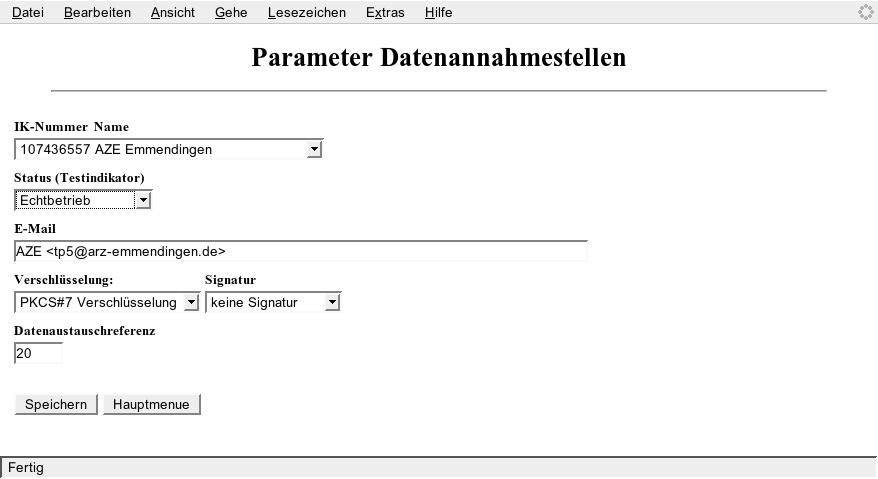
\includegraphics[width=80mm]{parameter_datenannahmestellen}
\caption{Maske Parameter der Datenannahmestellen\label{parameter:datenannahmestellen:fig}}
\end{figure}

Für jede Datenannahmestelle sind fünf Parameter zu erfassen, die in den
folgenden Tabellen beschrieben sind. Die Parameter enden alle mit der
IK Nummer der Datenannahmestelle, z.B. DTAUS104212516 oder 
IK104212516 bei Datenannahmestelle 
104212516. Bei Datenannahmestelle 661200093 wäre der Name des Parameters
IK661200093.

\begin{minipage}{14cm}
\begin{tabular}{|p{1cm}p{12cm}|}
\firsthline
\textbf{Name}&\textbf{Beschreibung}
\tabularnewline\hline
IK&
Mit welchen Status wird der Datenaustausch mit der Datenannahmestelle
durchgeführt. Name des Parameters z.B. IK104212516 bei Datenannahmestelle 
104212516. Sobald dieser Parameter für eine Datenannahmestelle gepflegt
ist, wird die Datenannahmestelle im Menue Rechnungsgenerierung angezeigt.
Wichtig ist es alle Parameter der Datenannahmestelle zu pflegen, um eine
korrekte elektronische Rechnung zu generieren. Trotz Pflege aller Parameter
besteht die Möglichkeit, dass eine Datennahmestelle in der Maske
Rechnungsgenerierung nicht als solche angezeigt wird, dies ist dann der
Fall, wenn kein öffentlicher Schlüssel der Datennahmestelle vorhanden ist.
\begin{enumerate}
\item[00] 
\index{Testphase}
Testphase gemäß \cite{pruefverfahren}. Diese Phase ist nur für
Softwareentwickler oder zum Test der Anwendung notwendig. Sie kann
auch genutzt werden, um zu prüfen, ob Rechnung akzeptiert werden.
\item[01] 
\index{Erprobungsphase}
Erprobungsphase gemäß \cite{pruefverfahren}. Dies ist die
Standardeinstellung in \tinyHeb\/ nach der Installation.
Mit jeder Datenannahmestelle muss die Erprobungsphase durchlaufen 
werden\footnote{mit fast jeder -- erreicht man die Zertifizierung bei einer AOK,
 so wird dies allen anderen AOKen in Deutschland mitgeteilt.}. In dieser
Phase müssen sowohl Papier- wie auch elektronische Rechnungen gestellt
werden. Auf der Papierrechnung wird ein entsprechender Hinweis mit
ausgegeben, dass diese Rechnung auch per E-Mail verschickt wurde. Dies
wird von einigen Datenannahmestellen so gewünscht. Die Erprobungsphase
ist beendet, wenn der Leistungserbringer von der Krankenkasse zum 
Echtverfahren zugelassen wird \cite{pruefverfahren}.
\item[02] 
\index{Echtverfahren}
Echtverfahren gemäß \cite{pruefverfahren}. Im Echtverfahren
ist es nicht mehr notwendig Rechnungen auf Papier zu verschicken.
Belege wie z.B. für Auslagen oder auch Rezepte sind weiterhin an die 
in der Kostenträgerdatei genannten 
Belegannahmestellen zu schicken. In \tinyHeb\/ wird weiterhin eine
Papierrechnung erstellt. Auf dieser ist vermerkt, dass diese ausschließlich
für die eigenen Unterlagen ist. Sind Urbelege zu verschicken, wird im Anschluß
an die Rechnung zusätzlich ein Formblatt für Begleitzettel für Urbelege 
generiert \cite{urbelege}. \index{Urbeleg} 
Auf diesem Formblatt kann eingetragen werden,
wie viele Urbelege verschickt werden.
\end{enumerate}
\tabularnewline\hline
\lasthline
\end{tabular}
\captionof{table}{Parameter für Datenaustausch\label{datenaus_parm_ik}}
\end{minipage}



\begin{minipage}{14cm}
%\centering
\begin{tabular}{|p{1cm}p{12cm}|}
\firsthline
\textbf{Name}&\textbf{Beschreibung}
\tabularnewline\hline
SCHL&
\index{Verschlüsselung}
Mit welchem Verschlüsselungsverfahren wird der Datenaustausch mit 
der Datennahmestelle durchgeführt, z.B. Name des Parameters SCHL661200093.
\begin{enumerate}
\item[00] Es wird keine Verschlüsselung durchgeführt. Sobald echte Daten
über das Internet ausgetausch werden, ist man gemäß Datenschutzgesetz dazu
verpflichtet, die Daten zu verschlüsseln. Das heißt, dieser Wert sollte nur
für Testzwecke mit ``Spieldaten'' gewählt werden.
\item[02] Verschlüsselung im PEM Verfahren. Dieses Verfahren ist nur bei
den gesetzlichen Krankenkassen in Deutschland gebräuchlich und wird von
\tinyHeb\/ nicht unterstützt. Bei diesem Verfahren wird von den 
Krankenkassen mit einer Schlüssellänge von 768 Bit gearbeitet. Diese Länge
wird vom BSI nicht mehr als sicher angesehen.
\item[03] 
\index{PKCS\#7}
Verschlüsselung im PKCS\#7 Format. Dieses Verfahren ist der Standard
für \tinyHeb\/ und wird der zukünftige Standard im Datenaustausch mit den
gesetzlichen Krankenkassen werden.
\end{enumerate}
\tabularnewline\hline
\lasthline
\end{tabular}
\captionof{table}{Parameter für Datenaustausch (Verschlüsselung)\label{datenaus_parm_schl}}
\end{minipage}



\begin{minipage}{13.0cm}
\begin{tabular}{|p{1.4cm}p{11.8cm}|}
\firsthline
\textbf{Name}&\textbf{Beschreibung}
\tabularnewline\hline
SIG&
\index{Signatur}
\index{Signieren|see{Signatur}}
Mit welchem Signaturverfahren wird der Datenaustausch mit 
der Datenannahmestelle durchgeführt, z.B. Name des Parameters SIG661200093
bei Datenannahmestelle 661200093.
\begin{enumerate}
\item[00] Die Rechnung wird mit keiner Signatur versehen. Die ist der
Standard in \tinyHeb, da aktuell die Datenannahmestellen nicht in der
Lage sind, signierte Rechnungen entgegenzunehmen. Dies entspricht nach
Meinung des Autors nicht dem SigG. Entsprechende Rechnung werden aber
anstandslos gezahlt.
\item[02] Signierung im PEM Verfahren. Dieses Verfahren ist nur bei
den gesetzlichen Krankenkassen in Deutschland gebräuchlich und wird von
\tinyHeb\/ nicht unterstützt.
\item[03] 
\index{PKCS\#7}
Signierung im PKCS\#7 Format. Dieses Verfahren ist in 
\tinyHeb\/ implementiert. Um eine Rechnung signieren zu können, ist es
notwendig über ein eigenes Zertifikat zu Verfügen, welches von der 
ITSG \cite{itsg} erteilt wird. Im Anhang in Abschnitt
\ref{anhang:eigenes_cert} ist beschrieben, wie Verfahren werden muss, um
ein solches Zertifikat zu erlangen. Dieser Abschnitt sollte im Detail
gelesen werden, da von der ITSG wenig Hilfe zu erwarten ist, wenn nicht
deren ``Tool'' D* genutzt wird.
\end{enumerate}
\tabularnewline\hline
\lasthline
\end{tabular}
\captionof{table}{Parameter für Datenaustausch (Signatur)\label{datenaus_parm_sig}}
\end{minipage}


\begin{minipage}{13.5cm}
\begin{table}[H]
\begin{tabular}{|p{1.3cm}p{11.9cm}|}
\firsthline
\textbf{Name}&\textbf{Beschreibung}
\tabularnewline\hline
MAIL&
An welche Mail Adresse müssen die Rechnungen bei der Datenannahmestelle 
geschickt werden, z.B. Name des Parameters MAIL661200093
bei Datenannahmestelle 661200093.
Hier muss die komplette E-Mail Adresse in Format: Name <email.datenannahmstelle.de> stehen.
D.h. für die Datenannahmestelle 661200093 Medent muss der Parameter folgenden
Wert enthalten: MEDENT <sole@datenannahme.medent.de>
\tabularnewline\hline
DTAUS&
Enthält die Datenaustauschreferenz für diese Datenannahmestelle, z.B. Name
des Parameters DTAUS661200093. Diese Parameter enthält die nächste zu
vergebene Austauschreferenz. Der Wert wird nachdem eine Rechnung
elektronisch verschickt wurde um eins erhöht. Wird eine neue
Datenannahmestelle parametrisiert, sollte dieser Wert auf eins gestellt
werden. Danach ist es nicht mehr nötig, diesen Wert manuell zu ändern.
\tabularnewline\hline
\lasthline
\end{tabular}
\captionof{table}{Parameter für Datenaustausch\label{datenaus_parm_mail}}
\end{table}
\end{minipage}

\paragraph{Beispiel für neue Datenannahmestelle}
Für die Datenannahmestelle Mendent gibt es unterschiedliche IK Nummern,
bisher ist nur die Datenannahmestelle mit der IK-Nummer 661200093
parametrisiert. D.h. es können nur elektronische Rechnungen an die
Techniker Krankenkasse geschickt werden, da diese auf o.g. Nummer
verweist.

Jetzt soll die Datenannahmestelle mit der IK Nummer 220910147
parametrisiert werden. D.h. es können zukünftig auch Rechnungen an
die KKH geschickt werden. Folgende Parameter müssen im Menue
Parameter neu erfasst werden:
\begin{table}[H]
\begin{tabular}{|p{3cm}|p{5cm}|p{5cm}|}
\firsthline
\textbf{Name}&\textbf{Beschreibung}&\textbf{Wert}
\tabularnewline\hline
IK220910147&
Datenannahmestelle (Medent w/ KKH)&
01
\tabularnewline\hline
DTAUS220910147&
Datenaustauschreferenz für diese Datenannahmestelle (hier Mendent w/ KKH)&
1
\tabularnewline\hline
SCHL220910147&
Verschlüsselung für Datenannahmestelle (hier Medent w/ KKH)&
03
\tabularnewline\hline
SIG220910147&
Signatur für Datenannahmestelle (hier Medent w/ KKH)&
00
\tabularnewline\hline
MAIL220910147&
Mail Adresse der Datenannahmestelle (hier Mendent w/ KKH)&
\nolinkurl{Medent <sole@datenannahme.medent.de>}
\tabularnewline\hline
\lasthline
\end{tabular}
\caption{Beispiel Parameter für neue Datenannahmestelle\label{beispiel_parm}}
\end{table}



\paragraph{Beispiel für eine zu ändernde Datenannahmestelle}
Mit der Datenannahmestelle ARZ-Emmendingen wurden bisher Rechnungen
im Rahmen der Erprobungsphase abgewickelt, d.h. der Parameter
IK107436557 hat den Wert 01. Nachdem nun drei Rechnungen erfolgreich
abgewickelt wurden, hat man eine E-Mail aus Emmendingen bekommen, die besagt,
Rechnungen dürfen zukünftig im Echtbetrieb verschickt werden.
D.h. der Wert zu Parameter IK107436557 muss auf 02  geändert werden.
Dazu wird der Parameter IK107436557 über die Maske ``Parameter suchen'' zur
Bearbeitung ausgewählt. Der Wert auf 02 geändert, im Pop-Down-Menue
``Ändern'' ausgewählt und der Knopf \knopf{Speichern} gedrückt. Das
wars, Emmendingen ist für den Echtbetrieb bereit. Alle anderen Parameter
zu dieser Datennahmestelle können identisch bleiben.

\section{Leistungsarten}\label{leistungsarten:abs}
Unter Leistungsarten werden in \tinyHeb\/ alle Punkte verstanden, die in
der Rechnung auftauchen sollen. Aus diesem Grund werden die Begriffe
Positionsnummer und Leistungsart häufig synonym verwendet.
Es ist möglich eigene Leistungsarten
zu definieren. Dies ist insbesondere sinnvoll für Arzneimittel, die
in der Rechnung unter Auslagen aufgeführt werden sollen. In den
Leistungsarten lässt sich definieren, ob bestimmte Plausiprüfungen bei
der späteren Erfassung von Rechnungsposten durchgeführt,
resp. ob weitere Leistungsarten automatisch angewählt werden sollen.
Die Leistungsarten sind vom Prinzip Parameter. In diesem Abschnitt
wird gezeigt, wie neue Leistungsarten angelegt, respektive geändert
werden können. Die Leistungsarten stellen ein mächtiges Werkzeug zur
Konfiguration der Anwendung dar. Allerdings besteht bei den Leistungsarten
noch mehr als bei den Parametern, die Möglichkeit zu einer nicht mehr
funktionierenden Anwendung zu gelangen. Es ist insb. zu beachten, dass
keinerlei Plausibilitätenprüfungen in der Maske Leistungsarten existieren.
Also: nur dann Leistungsarten
ändern, wenn man genau weiss, welche Auswirkung die Änderung hat.
\marginline{\Huge\bfseries!}%

\subsection{Leistungsartenerfassung}
\index{Leistungsarten}
\index{Positionsnummern}
Aus dem Hauptmenue gelangt man über den Link \nolinkurl{Leistungsarten}
in die Maske Leistungsarten (Abbildung \vref{leistungsarten:fig}).

\begin{figure}[h]
\centering
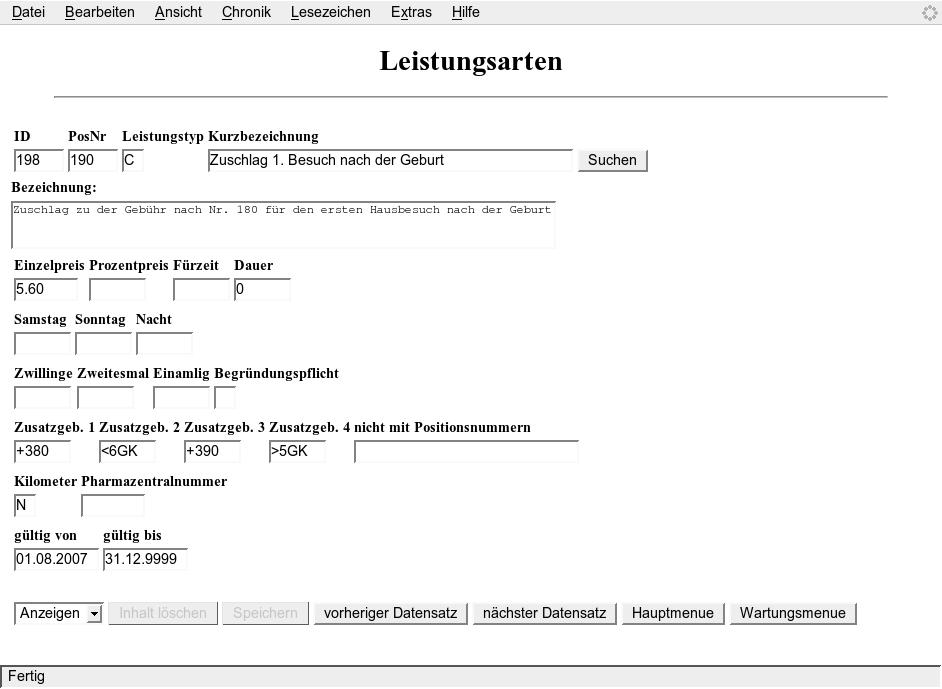
\includegraphics[width=80mm]{leistungsarten}
\caption{Leistungsarten\label{leistungsarten:fig}}
\end{figure}

Folgende Felder sind in der Maske vorhanden:
\begin{description}
\item[ID] Dieses Feld enthält die interne ID zum angezeigten Datensatz, das
Feld darf unter keinen Umständen geändert oder erfasst werden.
\item[PosNr] Dieses Feld enthält die offizielle Positionsnummer der
entsprechenden Leistung gemäß \cite{posnr} oder eine eigene nicht offizielle
Positionsnummer. Eigene Positionsnummern sind sinnvoll für Auslagen oder
Materialpauschalen. Es wird empfohlen für Materialpauschalen eine fortlaufende
3-stellige Nummer zu vergeben, die mit M beginnt, d.h. M001 bis M999. Der Inhalt
dieses Feldes wird zusammen mit dem Inhalt aus Feld \feld{Kurzbezeichnung}
in der Maske Rechnungsposten erfassen (siehe Abbildung 
\vref{rechnungspostenerfassen:fig}) im Feld \feld{PosNr:} angezeigt.
Analog wird der Inhalt des Feldes zusammen mit der Kurzbezeichnung auf
der Rechnung angedruckt.
\item[Leistungstyp] Dieses Feld enthält die Gruppe, der diese 
Leistungsart zugeordnet wird. Es sind fünf verschiedene Gruppen möglich:
\begin{enumerate}
\item[A] Mutterschaftsvorsorge,
\item[B] Geburt,
\item[C] Wochenbett,
\item[D] sonstige Leistungen,
\item[M] 
\index{Material}
Material, in Kombination mit dem Feld \feld{Zusatzgeb. 1} wird
entschieden, zu welcher Wirkstoffgruppe diese Materialie gehört. D.h. es
ist ein Wert zwischen 500 und 620 nach Hebammen-Vergütungsverordnung,
bzw. 76 und 88 nach HebGO zu erfassen. Wird im Feld \feld{Zusatzgeb. 1}
nichts erfasst, wird ``sonstige Auslagen (Positionsnummer 70 bzw. 800)'' 
angenommen.
\item[W] 
Wegegeld
\end{enumerate}

Anhand des Leistungstypes werden Plausibilitätenprüfungen in der
Rechnungserfassung durchgeführt, so sind Leistungen vom Typ A nur bis
zur Geburt des Kindes möglich und Leistungen vom Typ C nur ab der Geburt
des Kindes.

In der späteren Rechnung wird die erfasste Leistung entsprechend ihres
Leistungstypes in der jeweiligen Rubrik in der Rechnung angedruckt.

\item[Kurzbezeichnung] Dieses Feld enthält die Kurzbezeichnung der Leistung,
Diese Bezeichnung wird in der Maske Rechnungsposten erfassen im Feld
\feld{PosNr} und auf der späteren Rechnung angezeigt. Falls der
Leistungstyp ``M'' ist, wird diese Bezeichnung in die elektronische 
Rechnung übernommen\footnote{Entweder in Positionsnummer 800, bzw. 70, 
dies sind die einzigen
Positionsnummern, die unterschiedliche Bezeichnungen haben können.}.
\item[Bezeichnung] Dieses Feld enthält die ausführliche Beschreibung der
Leistungsart und wird in der weiteren Anwendung nicht genutzt.
\item[Einzelpreis] Dieses Feld enthält den Einzelpreis der Leistungsart.
Dieser Preis wird in der späteren Rechnung angedruckt und erscheint in
der Übersicht der erfassten Rechnungsposten in der Maske Rechnungserfassung.
Handelt es sich bei der Leistungsart um eine Leistung die nach Zeit (siehe
Feld \feld{Fürzeit}
abgerechnet wird, wird mit dem Wert aus diesem Feld multipliziert.
Falls die Leistung nur prozentual in Abhängigkeit einer anderen Leistung
berechnet werden soll, ist dieses Feld mit Null, resp. nicht zu befüllen.
Es ist zu beachten, dass in diesem Feld Dezimalstellen mit . (Punkt) und
nicht mit , (Komma) erfasst werden müssen, z.B.136.10 und nicht 136,10.
\item[Prozentpreis] Hier einen Wert einzutragen macht nur Sinn, wenn diese
Leistung in Abhängigkeit einer anderen Positionsnummer berechnet werden soll.
Ein Beispiel dafür ist Positionsnummer 18, bei der 25\% Zuschlag 
gerechnet werden müssen. Das Feld muss
für einen solchen Fall mit 0.25 gefüllt werden.
\item[Fürzeit] Über dieses Feld wird in der Anwendung gesteuert, ob eine
Leistungsart in Abhängigkeit der Zeit berechnet werden muss. In dieses
Feld ist die Zeit in Minuten einzutragen, für die jeweils abgerechnet wird.
Wird nur eine Zeit, z.B. 30 eingetragen, bedeutet dies, die Leistungsart
wird pro angefangene Zeit berechnet.
Z.B. bei Positionsnummer 4 ``Hilfe bei Beschwerden'' ist hier 30 
einzutragen, da jede angefangene halbe Stunde abgerechnet werden kann.
Muss die Leistungsart exakt abgerechnet werden, ist ein E vor der Minutenzahl
zu erfassen, z.B. E60. Dies ist z.B. bei Positionsnummer 8 der Fall, d.h.
die Position wird exakt auf 60 Minuten abgerechnet. In diesem Fall werden
auf der Rechnung die Minuten in Stunden umgerechnet und beides angedruckt.
Ist im Feld \feld{Fürzeit} ein Wert größer Null erfasst, werden bei Auswahl
der Positionsnummer in der Maske Rechnungserfassung die Felder
\feld{Uhrzeit von} und \feld{Uhrzeit bis} bis für die Erfassung freigeschaltet.
\item[Dauer] 
Dieses Feld sollte nur in Kombination mit dem \feld{Fürzeit}
erfasst werden. Ist der Wert gepflegt, wird in der Maske Rechnungserfassung
eine zusätzliche Plausiprüfung aktiv. Der dort erfasste Zeitraum
(Feld \feld{Uhrzeit bis} Minus Feld \feld{Uhrzeit von}) wird mit der hier 
angegebene Dauer verglichen, ist er größer, muss
eine Begründung im Feld \feld{Begründung} erfasst werden.
\item[Samstag] 
In diesem Feld kann auf eine andere Positionsnummer verwiesen
werden. Es wird in der Rechnungserfassung evaluiert, ob das Datum
der Leistungserbringung auf einen Samstag fällt\footnote{Samstag ist im
Sinne der Hebammengebührenordnung erst nach 12:00, dies wird berücksichtigt}.
Wenn dies der Fall ist und im Feld
\feld{Samstag} ein Wert größer Null enthalten ist, 
wird die erfasste Positionsnummer
durch die Positionsnummer im Feld \feld{Samstag} ersetzt. Positionsnummer 4
ist ein Beispiel für den beschriebenen Sachverhalt. 
Dem Nutzer wird die Substitution durch einen Hinweis angezeigt. 
Wird im Feld
\feld{Samstag} eine Positionsnummer mit einem führenden + (Plus) erfasst,
erfolgt keine Substituierung der Positionsnummer, statt dessen wird die
angegebene Positionsnummer zusätzlich ausgewählt. Positionsnummer 18 ist
ein Beispiel für den beschriebenen Sachverhalt. Dem Nutzer wird die
Subsitution durch einen Hinweis angezeigt.
\item[Sonntag] 
Für das Feld \feld{Sonntag} gilt eine analoge Beschreibung,
wie für das Feld \feld{Samstag}. Sonntag und Feiertag werden identisch
behandelt. Die Feiertage müssen allerdings zuvor in der Maske Feiertage
erfasst worden sein (siehe dazu \vref{feiertage:abs}).
\item[Nacht] 
Für das Feld \feld{Nacht} gilt eine analoge Beschreibung,
wie für die Felder \feld{Samstag} und \feld{Sonntag}. Nacht ist im Sinne
der Hebammengebührenordung zwischen 20:00 Uhr Abends und 08:00 Uhr Morgens.
\item[Zwillinge] 
Dieses Feld hat in der aktuellen Version keine Bedeutung. Es
ist dafür vorgesehen die Positionsnummer für  Zuschlag Zwillinge aufzunehmen.
Damit dieser Zuschlag automatisch in der Rechnungserfassung berücksichtigt
werden kann.
\item[Zweitesmal]
In diesem Feld kann auf eine andere Positionsnummer verwiesen
werden. Es wird in der Rechnungserfassung evaluiert, ob auf eine andere
Positionsnummer verwiesen wird.
Wenn dies der Fall ist und im Feld
\feld{Zweitesmal} ein Wert größer Null enthalten ist, 
wird die erfasste Positionsnummer
durch die Positionsnummer im Feld \feld{Zweitesmal} ersetzt. Positionsnummer 22
ist ein Beispiel für den beschriebenen Sachverhalt. 
Dem Nutzer wird die Substitution durch einen Hinweis angezeigt. 
\item[Einmalig]
In diesem Feld kann auf eine andere Positionsnummer verwiesen
werden. Es wird in der Rechnungserfassung evaluiert, ob auf eine andere
Positionsnummer verwiesen wird. Wenn dies der Fall ist und im Feld
\feld{Einmalig} eine Positionsnummer mit einem führenden + (Plus) erfasst,
wird die
angegebene Positionsnummer zusätzlich ausgewählt. Positionsnummer 22 ist
ein Beispiel für den beschriebenen Sachverhalt. Dem Nutzer wird die
Subsitution durch einen Hinweis angezeigt.
Wird die Positionsnummer ohne führendes Plus erfasst, wird die im Feld
\feld{Posnr} angegebene Positionsnummer ersetzt.
ersetzt.
\item[Begründungspflicht]
Falls in diesem Feld J angegeben ist, wird im Rahmen der Rechnungserfassung
evaluiert, ob eine Begründung erfasst wurde. Ist dies nicht der Fall,
wird dies mit einem Fehlerhinweis angezeigt und die Positionsnummer kann
nicht gespeichert werden. Positionsnummer 8 ist ein Beispiel für den
beschriebenen Sachverhalt.
\item[Zusatzgeb.1] 
Über das Feld \feld{Zusatzgeb.1} werden in Abhängigkeit des Leistungstyps
verschiedene Sachverhalte gesteuert.
\begin{enumerate}
\item{Leistungstyp ist M}\\
Falls es sich um Leistungstyp M (Material) handelt, kann über das Feld
\feld{Zusatzgeb.1} auf eine Wirkstoffgruppe verwiesen 
werden\footnote{Wird das
Feld nicht erfasst bei Leistungstyp M, wird Positionsnummer 70 (alte
Gebührenordnung), bzw. 800 (Hebammen-Vergütungsvereinbarung)
``sonstige Auslagen'' angenommen.}.
\item{Leistungstyp ist nicht M (Material) und Feld \feld{Zusatzgeb.2} ist leer}\\
Es wird im Rahmen der Rechnungserfassung geprüft, ob auf eine 
Materialie verwiesen wird. Ist dies der Fall und das Feld 
\feld{Zusatzgeb.1} ist mit einem führenden + (Plus) erfasst, wird diese
Positionsnummer zusätzlich ausgewählt.\\
Positionsnummer 2 ist ein Beispiel
für diesen Sachverhalt, es wird bei Positionsnummer 2 immer zusätzlich die
entsprechende Materialpauschale (Positionsnummer 71) angewählt.
\item{Leistungstyp ist nicht M (Material) und \feld{Zusatzgeb.2} ist nicht leer}\\
Die im Feld \feld{Zusatzgeb.1} angegebene Positionsnummer wird 
zusätzlich ausgewählt, wenn die Bedingung aus dem Feld \feld{Zusatzgeb.2}
erfüllt ist.\\
Positionsnummer 24 ist ein Beispiel für diesen Sachverhalt.
\end{enumerate}

\item[Zusatzgeb.2]
In diesem Feld, kann eine zusätzliche Bedingung zu dem Feld \feld{Zusatzgeb.1}
angegeben werden. Das Feld muss wie folgt erfasst werden:\\
\verb|{Operator}{Zahl}{Vergleichswert}| dabei darf der Operator aktuell nur
die Werte > (größer), < (kleiner) oder = (gleich) enthalten. Die Zahl darf
nur Werte zwischen 0 und 999 enthalten. Als Vergleichswert ist aktuell nur 
der Wert GK (Geburtsdatum Kind) vorgesehen.
\paragraph{Beispiel}
Bei Positionsnummer 24 handelt es sich um den Zuschlag 1. Besuch nach der
Geburt. Wenn dies der Fall ist, kann auch die entsprechende Materialpauschale
Positionsnummer 74 oder 75 gewählt werden. D.h. bedeutet, in Feld
\feld{Zusatzgeb.1} wird +75 erfasst, die Bedingung in Feld 
\feld{Zusatzgeb.2} >4GK, d.h. liegt der Tag des ersten Besuches mehr als vier
Tage nach der Geburt des Kindes, wird Positionsnummer 75 zusätzlich ausgewählt.
\item[Zusatzgeb.3]
Dieses Feld hat eine ähnliche Beschreibung wie Feld \feld{Zusatzgeb.1}, es
wird allerdings nur in Kombination mit Feld \feld{Zusatzgeb.4} genutzt.
Die hier angegeben Positionsnummer wird ausgewählt, wenn die Bedingung aus
Feld \feld{Zusatzgeb.4} erfüllt ist.
\item[Zusatzgeb.4]
In diesem Feld kann eine zusätzliche Bedingung zu dem Feld \feld{Zusatzgeb.3}
angegeben werden. Das Feld muss wie folgt erfasst werden:\\
\verb|{Operator}{Zahl}{Vergleichswert}| dabei darf der Operator aktuell nur
die Werte > (größer), < (kleiner) oder = (gleich) enthalten. Die Zahl darf
nur Werte zwischen 0 und 999 enthalten. Als Vergleichswert ist aktuell nur 
der Wert GK (Geburtsdatum Kind) vorgesehen.
\paragraph{Beispiel}
Bei Positionsnummer 24 handelt es sich um den Zuschlag 1. Besuch nach der
Geburt. Wenn dies der Fall ist, kann auch die entsprechende Materialpauschale
Positionsnummer 74 oder 75 gewählt werden. D.h. bedeutet, in Feld
\feld{Zusatzgeb.3} wird +74 erfasst, die Bedingung in Feld 
\feld{Zusatzgeb.4} <5GK, d.h. liegt der Tag des ersten Besuches weniger
als fünf
Tage nach der Geburt des Kindes, wird Positionsnummer 74 zusätzlich ausgewählt.
\item[nicht mit Positionsnummer]
In diesem Feld kann eine durch ``,'' Komma separierte Liste von
Positionsnummern angegeben werden, die nicht mit der aktuellen Positionsnummer
an einem Tag erfasst werden dürfen. Z.B. Positionsnummer 030 darf nicht mit
den Positionsnummern 010, 030 am gleichen Tag erfasst werden.
\item[Kilometer]
Über dieses Feld wird gesteuert, ob in der Maske Rechnungsposten erfassen,
die Felder \feld{Kilometer Tag} und \feld{Kilometer Nacht} für die Erfassung
freigeschaltet sind. Durch Eingabe von ``J'' werden die Felder freigeschaltet,
durch die Eingabe von ``N'' für die Erfassung gesperrt.
\item[Pharmazentralnummer]
\index{PZN|see{Pharmazentralnummer}}
\index{Pharmazentralnummer}
In diesem Feld muss die Pharmazentralnummer (PZN) bei Materialien angegeben
werden\footnote{ab 01.02.2008 ist es Pflicht die Pharmazentralnummer bei 
elektronischen Rechnungen zu übermitteln}. Diese Nummer ist auf den
Medikamentenpackungen aufgedruckt oder kann in der Apotheke erfragt werden.
\item[gültig von]
Dieses Feld gibt an, ab wann die Positionsnummer mit dieser Ausprägung 
gültig ist. Dies ist z.B. sinnvoll, wenn eine neue Gebührenordnung ab
einem bestimmten Zeitpunkt gilt. Eine Positionsnummer kann in der Maske
Rechnungsposten erfassen nur dann ausgewählt werden, wenn das aktuelle
Tagesdatum größer oder gleich dem Feld \feld{gültig von} ist und kleiner
oder gleich dem Feld \feld{gültig bis}.
\item[gültig bis]
Dieses Feld gibt an, bis wann die Positionsnummer mit dieser Ausprägung 
gültig ist. Dies ist z.B. sinnvoll, wenn eine alte Gebührenordnung nur
bis zu einem bestimmten Zeitpunkt gilt.
\end{description}


\subsection{Beschreibung der Knöpfe im Leistungsartenmenue}
\begin{description}
\item[Suchen] Mit dem Knopf \knopf{Suchen} kann eine weitere Maske geöffnet
werden, über die Leistungsarten gesucht werden können. Die Beschreibung zu der
Suchmaske befindet sich in Abschnitt \vref{leistungsartensuchen:abs}.
In diese Maske wird der Wert aus dem Feld \feld{Posnr} übernommen 
und die Suche unmittelbar gestartet.
\item[Inhalt löschen] Der Knopf \knopf{Inhalt löschen} ist nur dann
Aktiv, wenn in dem
Pop Down Menue vor dem Knopf der Wert Neu ausgewählt wurde. Wird der Knopf
gedrückt, werden alle Felder der Maske auf ihren inital Wert gesetzt und das
Pop Down Menue springt auf den Wert Anzeigen,
\item[Speichern/ Löschen] Der Knopf \knopf{Speichern} ist nur dann Aktiv,
wenn im Auswahlmenue entweder der Wert ``Neu'' oder ``Ändern'' gewählt wird. 
\par
Falls Neu 
ausgewählt wurde, wird eine neue Leistungsart in der Datenbank gespeichert
und das Pop Down Menue springt auf den Wert Anzeigen. Es finden die
identischen Plausiprüfungen, die schon bei den einzelnen Feldern
beschrieben wurden, statt.
\par
Falls Ändern gewählt wurde, wird der Datensatz, der sich in der Datenbank
befindet mit den angezeigten Werten überschrieben und das Pop Down Menue
springt auf den Wert Anzeigen. 
Es finden die
identischen Plausiprüfungen, die schon bei den einzelnen Feldern
beschrieben wurden,
statt.\par
Falls im Pop Down Menue Löschen ausgewählt wurde, erhält der Knopf die
Beschriftung Löschen. Durch Drücken des Knopfes wird der Datensatz aus der
Datenbank gelöscht. Es findet keine Plausiprüfung statt.
Wurde der Datensatz erfolgreich gelöscht, werden
alle Felder der Maske auf ihren Initial-Wert gesetzt und das Auswahlmenue
steht auf den Wert Anzeigen.
\item[vorheriger Datensatz] Dieser Knopf ist nur dann aktiv, wenn der Wert
des Pop Down Menues auf Anzeigen steht. Durch Drücken des Knopfes wird auf
den vorherigen Datensatz in der Datenbank gesprungen. Der vorherige Datensatz
ist derjenige mit der nächst kleineren Positionsnummer, 
als der aktuell angezeigte. Ist
man am ersten Datensatz angekommen, bleibt dieser in der Maske erhalten.
\item[nächster Datensatz] Dieser Knopf ist nur dann aktiv, wenn der Wert
des Pop Down Menues auf Anzeigen steht. Durch Drücken des Knopfes wird auf
den nächsten Datensatz in der Datenbank gesprungen. Der nächste Datensatz
ist derjenige mit der nächst höheren Positinsnummer, 
als der aktuell angezeigte. Ist
man am letzten Datensatz angekommen, bleibt dieser in der Maske erhalten.
\item[Hauptmenue] Über diesen Knopf gelangt man in die Maske Hauptmenue.
Dabei ist zu beachten, dass nicht überprüft wird, ob Änderungen oder neu
erfasste Daten gespeichert wurden. Es wird sofort in die Maske Hauptmenue
gesprungen.
\end{description}

Sind alle Felder erfasst, können die Daten gespeichert werden. Dazu ist
es notwendig im Pop Down Menue unten links den Wert 'Neu' auszuwählen.
Sobald dies geschehen ist, wird der Knopf \knopf{Speichern} aktiv 
geschaltet. Drückt man jetzt den Knopf \knopf{Speichern} werden die Daten
zu der Leistungsart permanent abgelegt. Nach dem Speichern wird die Auswahl im 
Pop Down Menue unten links auf den Wert 'Anzeigen' gesetzt.


\section{Leistungsarten suchen\label{leistungsartensuchen:abs}}
In diesem Absatz ist beschrieben, wie Leistungsarten im Datenbestand 
gesucht und ausgewählt werden können. Der  Aufruf erfolgt aus der 
Maske Leistungsarten (siehe Seite \pageref{leistungsarten:fig}) 
über den Knopf \knopf{Suchen}. 
Klickt man auf den Knopf \knopf{Suchen} wird ein neues Fenster mit der
Überschrift ``Leistungsarten suchen'' geöffnet\footnote{sollte das Fenster 
noch geöffnet sein, wird es in den Vordergrund des Bildschirms geholt.} 
(siehe Abbildung \vref{leistungsartensuchen:fig}). Über die Felder \feld{Posnr,
Kurzbezeichnung, Gültigkeit, Leistungstyp} ist es möglich 
Suchkriterien vorzugeben, d.h. es werden bei der Suche nur die Leistungsarten
ausgegeben, bei denen alle vorgegebenen Werte vorhanden sind. Dabei ist
folgendes für die Felder zu beachten:

\begin{figure}[ht]
\centering
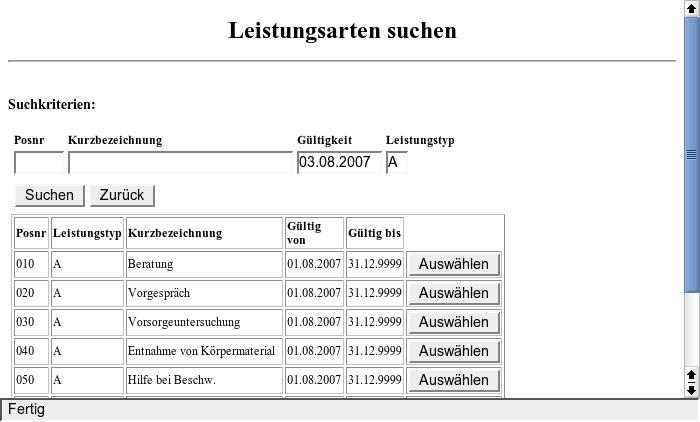
\includegraphics[width=9cm]{leistungsartensuchen}
\caption{Leistungsarten suchen\label{leistungsartensuchen:fig}}
\end{figure}

\begin{description}
\item[Posnr] 
Es wird nur nach den Leistungsarten gesucht, bei denen die Positionsnummer
exakt dem Feldes entspricht.
\item[Kurzbezeichnung] 
Es wird nur nach den Leistungsarten gesucht, bei denen die
Beschreibung mit dem Feldinhalt beginnt. Wird z.B. im Feld 
\feld{Kurzbezeichnung} ``Tel'' erfasst,
würden alle Leistungsarten, bei denen die Kurzbezeichnung mit ``Tel'' beginnt 
ermittelt werden, d.h. ``Telefon. Beratung im W.-Bett'' und ``Tel. Beratung
bei Stillschwierigk.''
\item[Gültigkeit]
Es wird nach den Leistungsarten gesucht, bei denen der Wert ``gültig von''
kleiner ist als der im Feld \feld{Gültigkeit}  erfasste Wert und
``gültig bis'' größer ist als der im Feld \feld{Gültigkeit} erfasste Wert.
Wird dieses Feld leer gelassen, wird automatisch mit dem Tagesdatum gesucht.
Um unabhängig vom Datum zu suchen, kann '*' oder '\%' erfasst werden.
In der Regel sollte man den Wert leer lassen.

\item[Leistungstyp] 
Es wird nur nach den Leistungsarten gesucht, bei denen der Leistungstyp
exakt der Vorgabe entspricht. D.h. wird hier ein ``C'' erfasst,
werden ausschließlich Positionsnummern aus dem Bereich Wochenbett
ermittelt.
\end{description}

Der Werte der Positionsnummer wird aus der Maske Leistungsarten
in die Suchkriterien übernommen und die Suche gestartet.
Die Felder können jederzeit mit neuen Kriterien gefüllt und die Suche
über den Knopf \knopf{Suchen} gestartet werden.

Das Ergebnis der Suche wird unmittelbar unter den Suchkriterien ausgegeben.
Es werden die Daten zu Positionsnummer, Leistungstyp, Kurzbezeichnung und
der Gültigkeitszeitraum ausgegeben.

Über den Knopf \knopf{Auswählen} werden die Daten der Leistungsart in die Maske
übernommen, aus der die Suchfunktion aufgerufen wurde. Die Maske
``Leistungsarten suchen''
wird danach geschlossen.

Falls keine Leistungsart den gewünschten Suchkriterien entspricht, 
kann entweder
durch Klicken des Knopfes \knopf{Zurück} die Maske ``Leistungsarten suchen''
geschlossen werden, oder es können andere Suchkriterien erfasst werden.




\section{Feiertage\label{feiertage:abs}}
\index{Feiertage}
Wie schon im Kapitel Installation beschrieben, gehören auch die Feiertage
im weitesten Sinne zu den Parametern, da über die Feiertage gesteuert
wird, ob an diesen Tagen Zuschläge berechnet, beziehungsweise bestimmte
Positionsnummern zu erfassen sind.
Aus dem Hauptmenue gelangt man über den Link \nolinkurl{Feiertage}
in die Maske Feiertage (Abbildung \vref{feiertage:fig}).

\begin{figure}[ht]
\centering
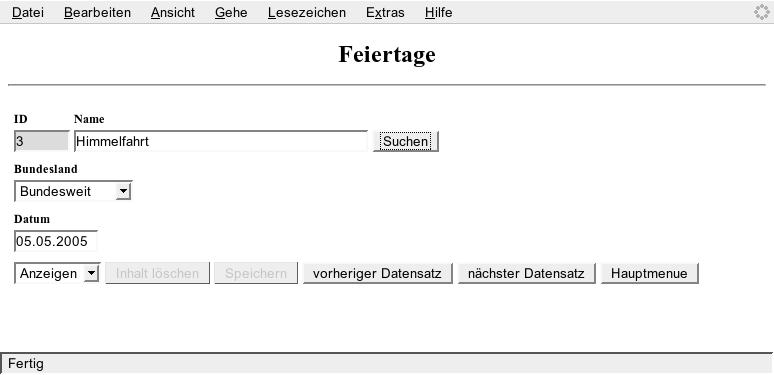
\includegraphics[width=80mm]{feiertage}
\caption{Feiertage\label{feiertage:fig}}
\end{figure}

Folgende Felder sind in der Maske vorhanden:
\begin{description}
\item[ID] 
Dieses Feld enthält die interne ID zum angezeigten Datensatz, es
kann nicht geändert oder erfasst werden.
\item[Name] 
Dieses Feld enthält die den Namen des Feiertages, z.B.
1. Weihnachtsfeiertag.
\item[Bundesland] 
Dieses Feld enthält das Bundesland in dem der Feiertag
\index{Bundesland}
gilt oder ``Bundesweit'', wenn es sich um einen Bundesweiten Feiertag
handelt. In der aktuellen Version von \tinyHeb\/ wird das Bundesland
bei der Ermittlung des Feiertages -- z.B. in der Rechnungserfassung -- 
nicht berücksichtigt\footnote{Dies wird sich in einer späteren
Version von \tinyHeb\/ ändern, schickt mir eine Mail, wenn Ihr die
Anforderung schon jetzt habt.}. D.h. es sollte bis auf weiteres immer
Bundesweit in dem Feld erfasst werden.
\item[Datum] 
Dieses Feld enthält das Datum des Feiertages. Die Erfasung muss im Format
TT.MM.JJJJ oder TT.MM.JJ erfolgen. Wird das Datum im Format TT.MM.JJ 
erfasst, erfolgt nach Verlassen des Feldes automatisch die Ermittlung
und Darstellung der 4-stelligen Jahreszahl. Ein ungültiges Datum führt
zu der Fehlermeldung: ``Bitte gültiges Datum erfassen''. Das Speichern
des Formulares mit ungültigen Werten ist nicht möglich.
\end{description}

\subsection{Beschreibung der Knöpfe im Feiertagemenue}
\begin{description}
\item[Suchen] Mit dem Knopf \knopf{Suchen} kann eine weitere Maske geöffnet
werden, über die Feiertage gesucht werden können. Die Beschreibung zu der
Suchmaske befindet sich in Abschnitt \vref{feiertagsuchen:abs}.
In diese Maske werden die Werte aus den Feldern \feld{Name, Bundesland} sowie
\feld{Datum} übernommen und die Suche unmittelbar gestartet.
\item[Inhalt löschen] Der Knopf \knopf{Inhalt löschen} ist nur dann
Aktiv, wenn in dem
Pop Down Menue vor dem Knopf der Wert ``Neu'' ausgewählt wurde. Wird der Knopf
gedrückt, werden alle Felder der Maske auf ihren Inital-Wert gesetzt und das
Pop Down Menue springt auf den Wert Anzeigen,
\item[Speichern/ Löschen] Der Knopf \knopf{Speichern} ist nur dann aktiv,
wenn im Auswahlmenue entweder der Wert ``Neu'' oder ``Ändern'' gewählt wird. 
\par
Falls ``Neu''
ausgewählt wurde, wird ein neuer Feiertag in der Datenbank gespeichert
und das Pop Down Menue springt auf den Wert Anzeigen. Es finden die
identischen Plausiprüfungen, die schon bei den einzelnen Feldern
beschrieben wurden, statt.
\par
Falls ``Ändern'' gewählt wurde, wird der Datensatz, der sich in der Datenbank
befindet mit den angezeigten Werten überschrieben und das Pop Down Menue
springt auf den Wert Anzeigen. 
Es finden die
identischen Plausiprüfungen, die schon bei den einzelnen Feldern
beschrieben wurden,
statt.\par
Falls im Pop Down Menue Löschen ausgewählt wurde, erhält der Knopf die
Beschriftung Löschen. Durch Drücken des Knopfes wird der Datensatz aus der
Datenbank gelöscht. Es findet keine Plausiprüfung statt.
Wurde der Datensatz erfolgreich gelöscht, werden
alle Felder der Maske auf ihren Initial-Wert gesetzt und das Auswahlmenue
steht auf den Wert Anzeigen.
\item[vorheriger Datensatz] Dieser Knopf ist nur dann aktiv, wenn der Wert
des Pop Down Menues auf Anzeigen steht. Durch Drücken des Knopfes wird auf
den vorherigen Datensatz in der Datenbank gesprungen. Der vorherige Datensatz
ist derjenige mit der nächst kleineren ID, als der aktuell angezeigte. Ist
man am ersten Datensatz angekommen, bleibt dieser in der Maske erhalten.
\item[nächster Datensatz] Dieser Knopf ist nur dann aktiv, wenn der Wert
des Pop Down Menues auf Anzeigen steht. Durch Drücken des Knopfes wird auf
den nächsten Datensatz in der Datenbank gesprungen. Der nächste Datensatz
ist derjenige mit der nächst höheren ID, als der aktuell angezeigte. Ist
man am letzten Datensatz angekommen, bleibt dieser in der Maske erhalten.
\item[Hauptmenue] Über diesen Knopf gelangt man in die Maske Hauptmenue.
Dabei ist zu beachten, dass nicht überprüft wird, ob Änderungen oder Neu
erfasste Daten gespeichert wurden. Es wird sofort in die Maske Hauptmenue
gesprungen.
\end{description}

Sind alle Felder erfasst, können die Daten gespeichert werden. Dazu ist
es notwendig im Pop Down Menue unten links den Wert 'Neu' auszuwählen.
Sobald dies geschehen ist, wird der Knopf \knopf{Speichern} aktiv 
geschaltet. Drückt man jetzt den Knopf \knopf{Speichern} werden die Daten
zu dem Feiertag permanent abgelegt. Nach dem Speichern wird die Auswahl im 
Pop Down Menue unten links auf den Wert 'Anzeigen' gesetzt.

\section{Feiertag suchen\label{feiertagsuchen:abs}}
In diesem Absatz ist beschrieben, wie Feiertage im Datenbestand gesucht und
ausgewählt werden können. Der  Aufruf erfolgt aus der 
Maske Feiertage (siehe Seite \pageref{feiertage:fig}) 
über den Knopf \knopf{Suchen}. 
Klickt man auf den Knopf \knopf{Suchen} wird ein neues Fenster mit der
Überschrift ``Feiertag suchen'' geöffnet\footnote{sollte das Fenster 
noch geöffnet sein, wird es in den Vordergrund des Bildschirms geholt.} 
(siehe Abbildung \vref{feiertagsuchen:fig}). Über die Felder \feld{Name,
Bundesland, Datum} ist es möglich 
Suchkriterien vorzugeben, d.h. es werden bei der Suche nur die Feiertage
ausgegeben, bei denen alle vorgegebenen Werte vorhanden sind. Dabei ist
folgendes für die Felder zu beachten:

\begin{figure}[ht]
\centering
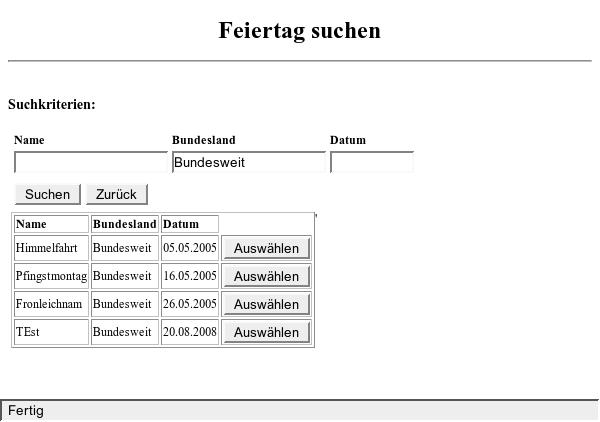
\includegraphics[width=9cm]{feiertagsuchen}
\caption{Feiertag suchen\label{feiertagsuchen:fig}}
\end{figure}

\begin{description}
\item[Name] 
Es wird nur nach den Feiertagen gesucht, bei denen der Name
einen Teil des Feldes enthält.
Wird z.B. im Feld \feld{Name} ``Weihn'' erfasst,
würde ``1. Weihnachtstag'' und ``2. Weihnachtstag'' ermittelt werden.
\item[Bundesland] 
Es wird nur nach den Feiertagen gesucht, bei denen die
Beschreibung mit dem Feldinhalt beginnt. Wird z.B. im Feld 
\feld{Bundesland} ``B'' erfasst,
würden alle Feiertage, bei denen das Bundesland mit ``B'' beginnt 
ermittelt werden, d.h. ``Bayern'' und ``Bundesweit''
\footnote{wobei in der aktuellen Version nur Bundesweit Sinn macht,}.
\item[Datum] Es wird nur nach den Feiertage gesucht, die diesen Wert
enthalten.
\end{description}

Die Werte Name und Bundesland
in die Suchkriterien übernommen und die Suche gestartet.
Die Felder können jederzeit mit neuen Kriterien gefüllt und die Suche
über den Knopf \knopf{Suchen} gestartet werden.

Das Ergebnis der Suche wird unmittelbar unter den Suchkriterien ausgegeben.
Es werden die Daten zu Name, Bundesland und Datum ausgegeben.

Über den Knopf \knopf{Auswählen} werden die Daten des Feiertages in die Maske
übernommen, aus der die Suchfunktion aufgerufen wurde. Die Maske
``Feiertag suchen''
wird danach geschlossen.

Falls keine Feiertage den gewünschten Suchkriterien entsprichen, kann entweder
durch Klicken des Knopfes \knopf{Zurück} die Maske ``Feiertag suchen''
geschlossen werden, oder es können andere Suchkriterien erfasst werden.


%%% Local Variables: 
%%% mode: latex
%%% TeX-master: t
%%% End: 
